\documentclass[11pt]{article}
\usepackage[margin=1in]{geometry}\usepackage{amsmath,amssymb,amsthm,booktabs,graphicx,hyperref}
\newtheorem{proposition}{Proposition}\newtheorem{definition}{Definition}
\title{Approximate Predictive Sufficiency of Local Chord Content: Roman Function as Applied-Chord Lumping and a Failed Preregistered MDL Repair}
\author{Anonymous}
\date{Draft, September 2026}
\begin{document}\maketitle

\begin{abstract}
Roman-numeral labels combine local chord content with functional category choices. We test, on the observed annotations of the Beethoven piano sonatas, the Annotated Beethoven Corpus quartets and the Mozart piano sonatas, whether $Z=(\text{chromatic relative root},\text{mode},\text{chord type})$ is operationally sufficient under a fixed prequential code at context depths $m=1,2$. The genuine refinement $F_{\mathrm{nested}}=(\text{numeral},\text{relative root},\text{mode},\text{chord type})$ deterministically contains $Z$. Across the base, root-free fixed-alphabet and clean-target analyses the residue $\Delta=L(Z)-L(F_{\mathrm{nested}})$ never exceeds 0.0487 bits per chord: the Beethoven sonatas at $m=1$ give 0.0454 to 0.0487 with 90.6 to 92.2\% of movements positive, while every ABC and Mozart value is at most 0.0127. All three corpora therefore meet our operational $\Delta\le 0.05$ criterion, with the Beethoven sonatas at the threshold at $m=1$. A selective label $F_{\mathrm{sel}}=(\text{numeral},\text{mode},\text{chord type})$ is not nested, because it groups applied dominants by function; its Beethoven contrast is 0.114/0.130 bits per chord, and relabelling only the applied chords by functional degree recovers 0.069/0.067, or 61\%/52\%, identifying a functional-lumping contribution rather than a nested syntax gain. A preregistered five-feature MDL repair of that contrast failed its joint recovery and stability rule. An integer-count certificate audits the mappings, folds and reported code lengths. All conclusions are restricted to these annotations, representations and coding protocols.
\end{abstract}

\part*{I. Logic}
\section{The representation question}
Two traditions describe tonal harmony: geometric accounts locate chords in voice-leading spaces (Tymoczko, 2006; Callender, Quinn and Tymoczko, 2008), functional accounts describe progressions with key-relative Roman labels (Rohrmeier, 2011). A predictive sufficiency comparison between them is valid only when the richer representation is a genuine refinement of the baseline. Our primary question is therefore whether the local-content state $Z$ is operationally sufficient, at a threshold of $0.05$ bits per chord, relative to a Roman representation that deterministically contains $Z$. Our secondary question concerns a different object: the selective label $F_{\mathrm{sel}}$, which does not contain the chromatic relative root and instead re-partitions applied chords by function; its code gain cannot be interpreted through the nested sufficiency proposition, so we analyse it as a representation effect and ask how much of the displayed contrast is recovered by functional relabelling of applied chords. Finally we report the confirmatory failure of a preregistered MDL repair intended to approximate that selective-label contrast. The contributions are the corrected nested measurement, the same-arity applied-chord attribution, the preregistered negative result and an auditable integer-count certificate. The original hypothesis of this study, a substantial Roman residue beyond a strong tonal baseline, was preregistered at $0.05$ bits per chord and failed.

\section{States, targets and quotients}
A chord event $t$ in a movement has a pitch-class set, an analysed root, a local key and a Roman label from the DCML annotation standard (Hentschel et al., 2021). A \emph{transition} from event $t$ to $t{+}1$ is canonicalised under common transposition: in the root-anchored version the previous root is sent to $0$; in the \emph{root-free} version the previous pitch-class set is sent to its lexicographically smallest transposition, so no analytic decision enters the geometry. A transition records the normalised previous set, the interval or shift to the next set, the normalised next set and the minimal total pitch-class displacement between the two sets.
\begin{definition}[contexts]
$G_t=O_m(t)$ is the tuple of the previous $m$ transitions (geometry). $K_t$ adds the root scale degree in the \emph{global} key, chord type and global mode. Let $Z_t=(r_t,\mu_t,\tau_t)$ with $r_t$ the chromatic root degree relative to the local tonic, $\mu_t$ the local mode and $\tau_t$ the chord type. The genuine refinement is $F_{\mathrm{nested},t}=(\nu_t,\rho_t,\mu_t,\tau_t)$ with $\nu_t$ the numeral and $\rho_t$ the relative root; the projection $h(\nu,\rho,\mu,\tau)=(r,\mu,\tau)$ recovers $Z_t$, so the sufficiency proposition applies. Separately, $F_{\mathrm{sel},t}=(\nu_t,\mu_t,\tau_t)$: no function recovers $Z_t$ from it (an applied $V/V$ has numeral $V$ but relative root degree $2$), so $F_{\mathrm{sel}}$ is a non-nested re-partition of $Z$ and $L(Z)-L(F_{\mathrm{sel}})$ is reported only as a coding contrast. The target $Y_t$ is the next transition; the \emph{no-current-shape} target keeps only the root shift and the displacement cost.
\end{definition}
$Z=h(F_{\mathrm{nested}})$ holds on every observed label combination (machine-checked; zero counterexamples); it does not hold for $F_{\mathrm{sel}}$.

\section{Sufficiency and repair}
Write $R_X=\inf_q \mathbb E[-\log_2 q(Y\mid G,X)]$ for the optimal log loss under context $X$.
\begin{proposition}[predictive sufficiency; standard]
If $Z=h(F)$ then $R_Z-R_F = H(Y\mid G,Z)-H(Y\mid G,F) = I(Y;F\mid G,Z)\ge 0$, and the following are equivalent: (i) $R_Z=R_F$; (ii) $Y\perp F\mid (G,Z)$; (iii) all fine states inside each $(G,Z)$ block share one predictive kernel; (iv) the projection $(G,F)\mapsto(G,Z)$ is predictively lumpable for $Y$.
\end{proposition}
\begin{proposition}[repair decomposition; standard]
For any repair $R=r(F)$ refining $Z$, $I(Y;F\mid G,Z)=I(Y;R\mid G,Z)+I(Y;F\mid G,R)$. On finite support, the classes of $(g,f)\equiv(g',f')\iff g=g',\,h(f)=h(f'),\,\widehat P(Y\mid g,f)=\widehat P(Y\mid g',f')$ form the unique coarsest refinement of $(G,Z)$ with zero empirical residue.
\end{proposition}
Both statements are background identities (log-loss regret equals conditional mutual information; kernel equality is Kemeny--Snell lumpability), not contributions of this paper. Their role is to fix what is being measured. The reported code-length differences are prequential estimates of $I(Y;F\mid G,Z)$; unlike the oracle quantity they can be negative, because a finite coder pays for every refinement it cannot fill with counts. We calibrate $\epsilon$-sufficiency with Pinsker: $I\le\epsilon$ implies $\mathbb E[\mathrm{TV}(P(Y\mid G,F),P(Y\mid G,Z))]\le\sqrt{\epsilon\ln 2/2}$, about $0.13$ at $\epsilon=0.05$.

\section{Exact certificate}
At submission every table will be regenerated from an archived manifest containing, for each corpus, $m$, target and context: for each corpus, $m$, target and context the counts $n_{gfy},n_{gf},n_{gzy},n_{gz}$, the cross-product audit $n_{gfy}n_{gz}=n_{gzy}n_{gf}$ per supported cell, the coding ledger (context, back-off level, counts, alphabet, UNK events, predictive probability, per-event loss), the exact code ratio $Q=\prod_t p_F(y_t)/p_Z(y_t)$ with $\log_2Q/N=L_Z/N-L_F/N$, one $Q_i$ per movement, and the repair fold files. The build fails if any headline number changes. Until the archive and its hashes are public this is an intended certificate, not a released one.

\part*{II. Experiment}
\section{Corpora and coder}
DCML corpora: Annotated Beethoven Corpus (70 quartet movements), Mozart piano sonatas (54), Beethoven piano sonatas (64). Events with a parseable numeral, chord tones and local key are kept; consecutive identical pitch-class sets are collapsed to chord changes (a no-collapse control follows). The coder is prequential: the geometry-only predictor is a Krichevsky--Trofimov estimator over the transition alphabet; every label-augmented context backs off to it with escape mass $\beta$ ($p=(c_{\mathrm{ctx}}(y)+\beta p_G(y))/(n_{\mathrm{ctx}}+\beta)$). Each movement is coded with counts from all other movements and updated within itself. Plain KT without back-off inverts every ranking (adding any label costs bits) and is reported as the sparsity control it is.

\begin{table}[t]\centering\small
\caption{Corrected nested comparison. Each entry is $\Delta=L(Z)-L(F_{\mathrm{nested}})$ in bits per chord, followed by the share of movements with positive residue. The maximum observed nested residue is 0.0487; all rows meet the operational $\Delta\le0.05$ criterion. Small negative finite-code contrasts do not contradict the oracle inequality.}\label{tab:nested}
\begin{tabular}{llrrr}\toprule corpus & $m$ & base nested & root-free + fixed alphabet & clean target \\ \midrule
Beethoven piano sonatas & 1 & 0.0454 (91\%) & 0.0466 (92\%) & 0.0487 (92\%) \\
Beethoven piano sonatas & 2 & 0.0169 (80\%) & 0.0114 (73\%) & 0.0130 (75\%) \\
ABC quartets & 1 & 0.0069 (66\%) & 0.0103 (70\%) & 0.0127 (74\%) \\
ABC quartets & 2 & -0.0022 (57\%) & 0.0024 (61\%) & 0.0037 (67\%) \\
Mozart piano sonatas & 1 & 0.0044 (72\%) & 0.0064 (76\%) & 0.0069 (76\%) \\
Mozart piano sonatas & 2 & -0.0003 (72\%) & 0.0005 (72\%) & 0.0008 (72\%) \\
\bottomrule\end{tabular}\end{table}

\begin{table}[t]\centering\small
\caption{Full corpora, root-anchored geometry, $\beta=1$. Bits per eligible chord; residue $=L(Z)-L(F_{\mathrm{sel}})$; last column = movements with positive residue.}\label{tab:full}
\begin{tabular}{llrrrrrrr}\toprule corpus & $m$ & $n$ & $G$ & $K$ (global key) & $Z$ (local key) & $F_{\mathrm{sel}}$ & residue & positive \\ \midrule
ABC quartets & 1 & 24140 & 5.777 & 5.191 & 4.735 & 4.723 & 0.012 & 51\% \\
ABC quartets & 2 & 24070 & 7.441 & 6.525 & 6.046 & 6.006 & 0.040 & 76\% \\
ABC quartets & 3 & 24000 & 8.613 & 7.710 & 7.303 & 7.258 & 0.045 & 76\% \\
Mozart sonatas & 1 & 13947 & 4.659 & 3.917 & 3.528 & 3.525 & 0.003 & 57\% \\
Mozart sonatas & 2 & 13893 & 5.930 & 4.724 & 4.265 & 4.240 & 0.025 & 72\% \\
Mozart sonatas & 3 & 13839 & 7.003 & 5.663 & 5.096 & 5.065 & 0.032 & 70\% \\
Beethoven sonatas & 1 & 19205 & 5.301 & 4.519 & 4.180 & 4.066 & 0.114 & 78\% \\
Beethoven sonatas & 2 & 19141 & 6.765 & 5.494 & 5.072 & 4.942 & 0.130 & 86\% \\
Beethoven sonatas & 3 & 19077 & 7.848 & 6.466 & 6.000 & 5.882 & 0.118 & 86\% \\
\bottomrule\end{tabular}\end{table}

\section{Controls}
\begin{table}[t]\centering\small
\caption{Residue $L(Z)-L(F_{\mathrm{sel}})$ under each control (bits/chord). The complete-label rows are negative because the finite coder cannot fill the refined contexts, not because the oracle information is negative.}\label{tab:ctrl}
\begin{tabular}{lrrrr}\toprule control & sonatas $m{=}1$ & $m{=}2$ & ABC $m{=}1$ & $m{=}2$ \\ \midrule
base & 0.114 & 0.130 & 0.012 & 0.040 \\
root-free geometry & 0.086 & 0.096 & -0.000 & 0.032 \\
no event collapse & 0.114 & 0.126 & 0.011 & 0.035 \\
fixed alphabet + UNK & 0.116 & 0.130 & 0.013 & 0.040 \\
target without current shape & 0.056 & 0.047 & -0.003 & 0.008 \\
smoothing $\beta=0.25$ & 0.138 & 0.116 & 0.019 & 0.028 \\
smoothing $\beta=4$ & 0.108 & 0.144 & 0.017 & 0.053 \\
complete Roman label & 0.006 & -0.096 & -0.185 & -0.268 \\
root-free + fixed + complete & 0.052 & -0.062 & -0.146 & -0.216 \\
\bottomrule\end{tabular}\end{table}
Figure~1 shows the same numbers as a forest; Figure~2 the share of movements with positive residue. Considered separately, root-free geometry retains 75\% and 74\% of the base sonata residue and the no-current-shape target retains 49\% and 36\%; under the combined root-free, fixed-alphabet, no-current-shape held-out protocol the sonata residues are 0.0486 and 0.0122 bits per chord. The ABC residue stays at or below $0.053$ under every control.

\begin{figure}[t]\centering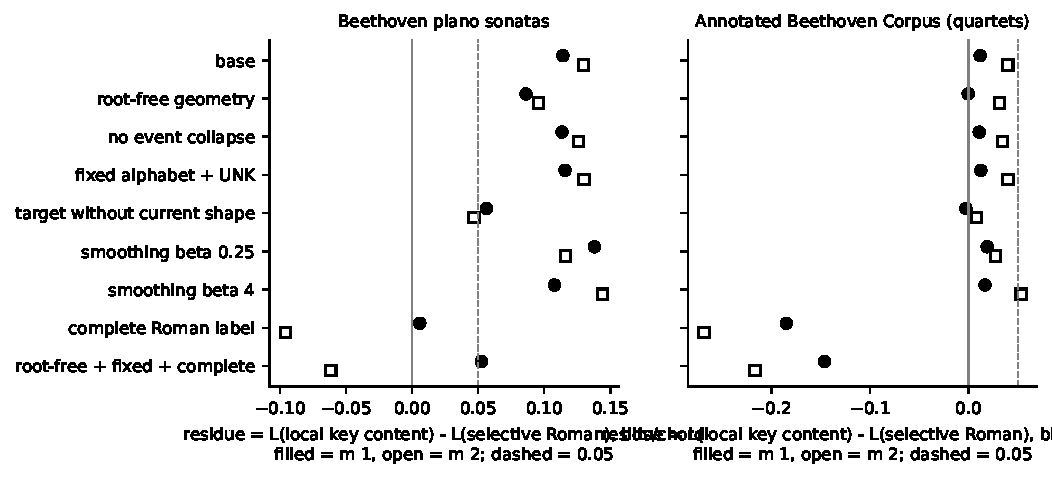
\includegraphics[width=\linewidth]{figs/fig1_controls.pdf}\caption{Control forest for the non-nested selective contrast $L(Z)-L(F_{\mathrm{sel}})$ (a coding contrast, not a sufficiency residue). Filled = $m{=}1$, open = $m{=}2$; dashed = $0.05$ bits/chord. The valid nested comparison is Table~\ref{tab:nested}: $F_{\mathrm{nested}}\to Z$ is a functional projection, whereas no projection exists from $F_{\mathrm{sel}}$ to $Z$ (an applied $V/V$ has numeral $V$ but relative root degree $2$).}\end{figure}
\begin{figure}[t]\centering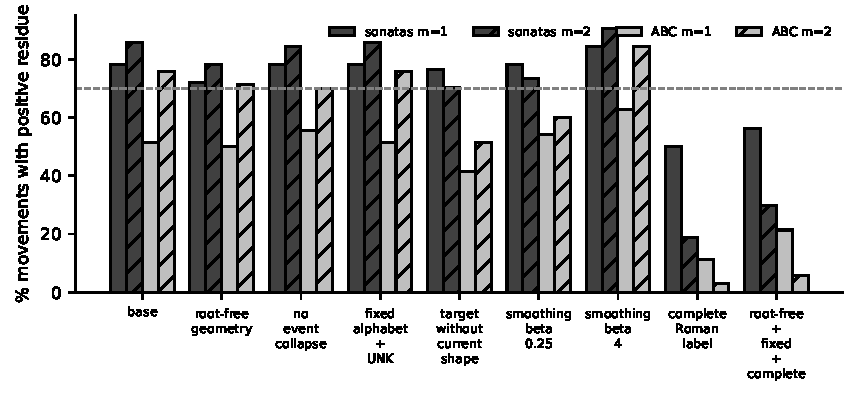
\includegraphics[width=\linewidth]{figs/fig2_prevalence.pdf}\caption{Share of movements with positive residue under each control.}\end{figure}

\section{What the selective-label contrast is}
The tuple (numeral, chord type, mode), at the same arity as $Z$, reproduces the Beethoven selective contrasts of 0.114/0.130 bits per chord exactly (0.114 and 0.130). This tuple is not a refinement of $Z$: it groups applied dominants onto their functional numeral while retaining spelled alterations elsewhere. Relabelling only the applied chords by functional degree, again at the same arity, yields gains of 0.069/0.067 bits per chord, equal to 61\%/52\% of the full selective contrast; the remaining 0.045/0.063 bits are not explained by this operation. Adding single complete-label fields on top of $Z$ recovers less (Figure~3): relative root 0.046/0.017, applied flag 0.026, spelled degree alone 0.037; inversion figures cost -0.036/-0.100. The supported positive finding is therefore that functional labelling gains predictive compression substantially through category lumping of applied chords, not that a nested Roman label supplies additional syntax.
\begin{figure}[t]\centering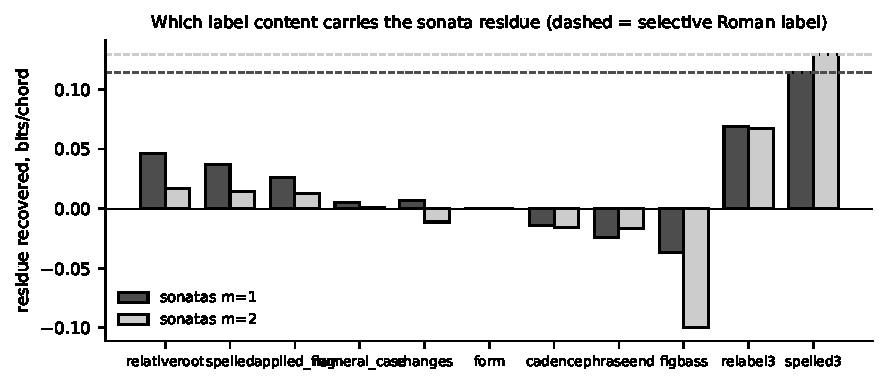
\includegraphics[width=\linewidth]{figs/fig3_attribution.pdf}\caption{Residue recovered by adding one label feature to $Z$ (Beethoven sonatas); dashed = selective label.}\end{figure}

\section{A failed preregistered MDL repair}
The preregistered MDL experiment attempted to approximate the observed $F_{\mathrm{sel}}$ coding contrast with a five-feature lattice. Because $F_{\mathrm{sel}}$ is non-nested, this is a predictive reconstruction test for a particular label re-partition, not a repair of a conditional syntax residue. Five feature blocks are parsed from the complete label: spelled degree $S$, case $C$, mixture $M$, applied structure $A$, inversion $I$. All 32 subsets are scored prequentially on training works, charged $D(B)=3+\lceil\log_2\binom{5}{|B|}\rceil$ bits, and the minimiser is applied to held-out works (5 folds grouped by work, SHA256 round robin). \begin{table}[t]\centering\small
\caption{Preregistered MDL repair over the 32-node lattice $\{S,C,M,A,I\}$, work-grouped 5-fold. $G_{\mathrm{ref}}=L(Z)-L(F_{\mathrm{sel}})$; $G_{\mathrm{repair}}$ is net of description cost; $\rho=G_{\mathrm{repair}}/G_{\mathrm{ref}}$; the preregistered rule required $\rho\ge0.80$ at both $m=1,2$ plus 4-of-5 fold stability; it failed because clean $m=1$ reached only 0.742 without stability and the base-target recoveries were 0.295 and 0.103. Recovery is n/a where $G_{\mathrm{ref}}\le 0$.}\label{tab:repair}
\begin{tabular}{llllrrrl}\toprule corpus & $m$ & target & $G_{\mathrm{ref}}$ & $G_{\mathrm{repair}}$ & $\rho$ & selected per fold & stable \\ \midrule
beethoven & 1 & clean & 0.049 & 0.036 & 0.742 & CMAI, SCMI, SCMAI, SCMAI, SCMAI & no \\
beethoven & 1 & base & 0.124 & 0.036 & 0.295 & MA, S, S, S, S & yes \\
beethoven & 2 & clean & 0.012 & 0.018 & 1.466 & SCMAI, SCMAI, SCMAI, SCMAI, SCMAI & yes \\
beethoven & 2 & base & 0.125 & 0.013 & 0.103 & S, S, S, S, S & yes \\
ABC & 1 & clean & -0.003 & 0.004 & n/a & SCMA, SCMA, SCMA, MA, MA & no \\
ABC & 1 & base & 0.015 & -0.001 & -0.034 & SCMA, SCMA, SCMA, SCMA, SCMA & yes \\
ABC & 2 & clean & 0.007 & 0.002 & 0.274 & SCMA, SCMA, SCMA, S, SCMA & yes \\
ABC & 2 & base & 0.039 & -0.002 & -0.046 & M, none, none, none, none & yes \\
\bottomrule\end{tabular}\end{table}
\begin{figure}[t]\centering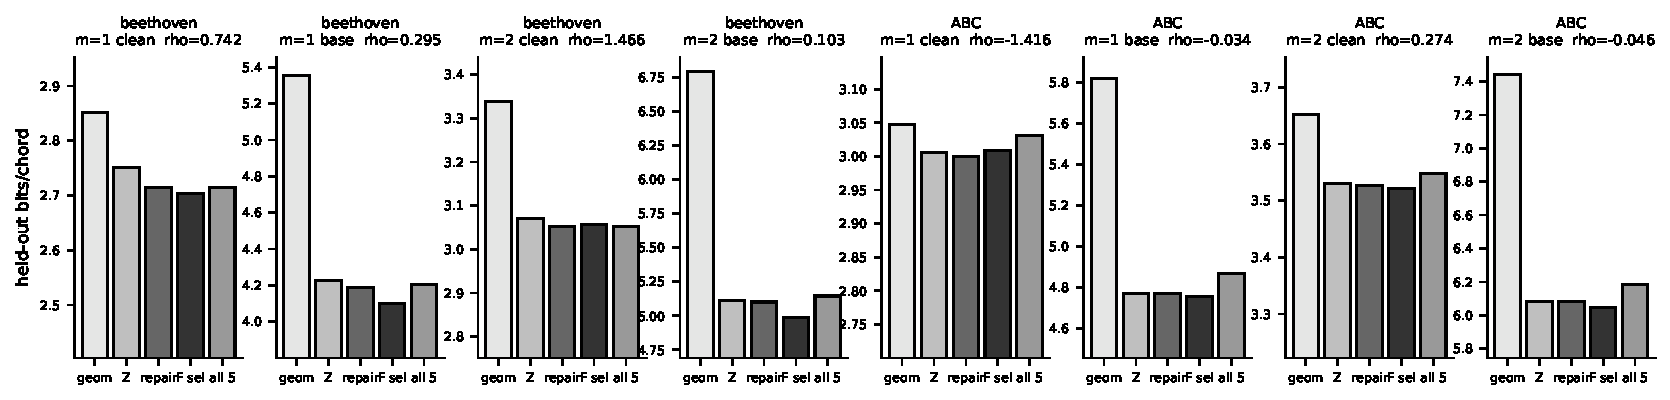
\includegraphics[width=\linewidth]{figs/fig4_repair.pdf}\caption{Held-out bits per chord for geometry, $Z$, the selected repair, the selective label and all five features.}\end{figure}

\section{Transfer and an out-of-domain contrast}
Training the coder on one corpus and coding another, sonata-target residues remain the largest under both adapted and source-only scoring, and the other targets stay at or below $0.053$ (Table~\ref{tab:tr}; adapted = counts updated on the target stream, source-only = frozen counts). In the Weimar Jazz Database (456 solos, chord symbols, no Roman labels) key-relative chord content improves next-move prediction by 2.43 bits per chord at $m=2$, four to five times the classical gain; the gain ranges from 2.12 (bebop) to 2.80 (postbop) across styles. Roman residue is undefined there; the contrast bounds how idiom-specific the classical numbers are.
\begin{table}[t]\centering\small\caption{Cross-corpus transfer of the residue (bits/chord).}\label{tab:tr}
\begin{tabular}{lrr}\toprule train $\rightarrow$ test, $m$ & adapted & source-only \\ \midrule
ABC$\rightarrow$beethoven m=1 & 0.110 & 0.103 \\
ABC$\rightarrow$beethoven m=2 & 0.146 & 0.122 \\
ABC$\rightarrow$mozart m=1 & -0.001 & 0.012 \\
ABC$\rightarrow$mozart m=2 & 0.032 & 0.048 \\
beethoven$\rightarrow$ABC m=1 & 0.018 & 0.037 \\
beethoven$\rightarrow$ABC m=2 & 0.053 & 0.052 \\
beethoven$\rightarrow$mozart m=1 & 0.007 & 0.037 \\
beethoven$\rightarrow$mozart m=2 & 0.029 & 0.047 \\
mozart$\rightarrow$ABC m=1 & 0.011 & 0.001 \\
mozart$\rightarrow$ABC m=2 & 0.044 & 0.034 \\
mozart$\rightarrow$beethoven m=1 & 0.100 & 0.066 \\
mozart$\rightarrow$beethoven m=2 & 0.123 & 0.068 \\
\bottomrule\end{tabular}\end{table}
\begin{table}[t]\centering\small\caption{WJazzD, $m=2$: key-relative content gain over geometry by style.}\label{tab:jz}
\begin{tabular}{lrrrr}\toprule style & $n$ & $G$ & $K$ & gain \\ \midrule
POSTBOP & 9170 & 5.168 & 2.370 & 2.799 \\
FUSION & 653 & 4.698 & 1.967 & 2.731 \\
COOL & 3894 & 4.952 & 2.560 & 2.392 \\
TRADITIONAL & 725 & 6.499 & 4.235 & 2.264 \\
SWING & 3005 & 5.287 & 3.027 & 2.260 \\
HARDBOP & 6256 & 4.317 & 2.156 & 2.161 \\
BEBOP & 3180 & 4.954 & 2.835 & 2.118 \\
\bottomrule\end{tabular}\end{table}
\begin{figure}[t]\centering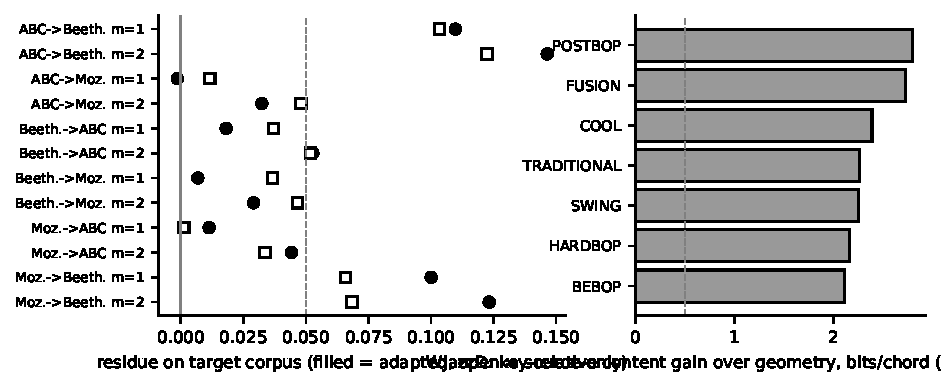
\includegraphics[width=\linewidth]{figs/fig5_transfer_jazz.pdf}\caption{Left: transfer residues (filled adapted, open source-only). Right: WJazzD key-relative gain by style; dashed = classical 0.5.}\end{figure}

\section{Scope and limitations}
Every claim in this study is descriptive of the observed annotations, fixed representations, folds, targets and prequential coder. The work-level non-nested Beethoven-versus-other margins are 0.1012/0.0904 bits per chord and the clean Beethoven residues 0.0425/0.0154, but the 21-work betting processes against $H_0{:}\mathbb E[d]\le0.05$ attained only $E_{\max}=0.714/0.7$, far below the rejection threshold of 20. We therefore make no claim about composers, styles, unobserved works or any population; because the 70 ABC movements are also Beethoven movements, no contrast here can be attributed to composer. Learned-model robustness was not tested; coder dependence remains a limitation (plain KT without back-off inverts the ranking, and the selective contrast moves between 0.138 and 0.108 bits at $m=1$ as the smoothing mass varies from 0.25 to 4).

\end{document}
